
%(BEGIN_QUESTION)
% Copyright 2006, Tony R. Kuphaldt, released under the Creative Commons Attribution License (v 1.0)
% This means you may do almost anything with this work of mine, so long as you give me proper credit

Acetic acid has a specific gravity of 1.0492$^{20/4}$.  Explain what the superscript ``20/4'' means, and calculate how much hydrostatic pressure a vertical column of acetic acid 12.3 meters high is supposed to produce, in PSI at 20$^{o}$ C.

$$\includegraphics[width=15.5cm]{i00231x01.eps}$$

$P$ = \underbar{\hskip 50pt} PSI

\vskip 10pt

Suppose the pressure gauge connected to the bottom of this vessel registers 14.2 PSI instead of the value you calculated.  Identify the likelihood of each specified fault shown in the table, considering each fault one at a time (i.e. no coincidental faults) to determine whether or not each fault could independently account for the discrepancy in pressure measurement.

% No blank lines allowed between lines of an \halign structure!
% I use comments (%) instead, so that TeX doesn't choke.

$$\vbox{\offinterlineskip
\halign{\strut
\vrule \quad\hfil # \ \hfil & 
\vrule \quad\hfil # \ \hfil & 
\vrule \quad\hfil # \ \hfil \vrule \cr
\noalign{\hrule}
%
% First row
{\bf Fault} & {\bf Possible} & {\bf Impossible} \cr
%
\noalign{\hrule}
%
% Another row
Gauge has a zero error &  &  \cr
%
\noalign{\hrule}
%
% Another row
Gauge has a span error &  &  \cr
%
\noalign{\hrule}
%
% Another row
Gauge has a linearity error &  &  \cr
%
\noalign{\hrule}
%
% Another row
Gauge has a hysteresis error &  &  \cr
%
\noalign{\hrule}
%
% Another row
Liquid inside tank is denser than acetic acid &  &  \cr
%
\noalign{\hrule}
%
% Another row
Level of liquid inside tank is less than what is shown in the diagram &  &  \cr
%
\noalign{\hrule}
} % End of \halign 
}$$ % End of \vbox


\vskip 20pt \vbox{\hrule \hbox{\strut \vrule{} {\bf Suggestions for Socratic discussion} \vrule} \hrule}

\begin{itemize}
\item{} Explain how we could determine what kind of calibration error this gauge had, if indeed its calibration was off at all.
\item{} Identify some alternative level-measurement technologies which could be used to sense liquid level in this vessel, which aren't affected by changes in liquid density.
\end{itemize}

\underbar{file i00231}
%(END_QUESTION)





%(BEGIN_ANSWER)

The 20/4 superscript means is that acetic acid is this much denser at 20$^{o}$ C than water is at 4$^{o}$ C.

%(END_ANSWER)





%(BEGIN_NOTES)

First, calculating the hydrostatic pressure as if the column were water instead of acetic acid:

\vskip 10pt

(12.3 m)(100 cm / 1 m)(1 inch / 2.54 cm)(1 PSI / 27.6807 "W.C.) = 17.494 PSI

\vskip 10pt

Now, correcting for acetic acid's specific gravity of 1.0492:

\vskip 10pt

(17.494 PSI)(1.0492 "W.C. / "acid) = 18.355 PSI

\vskip 10pt

Since this calculate figure for acid pressure (18.355 PSI) is considerably more than the 14.2 PSI indicated by the pressure gauge, we are left with these possibilities:

\vskip 10pt

% No blank lines allowed between lines of an \halign structure!
% I use comments (%) instead, so that TeX doesn't choke.

$$\vbox{\offinterlineskip
\halign{\strut
\vrule \quad\hfil # \ \hfil & 
\vrule \quad\hfil # \ \hfil & 
\vrule \quad\hfil # \ \hfil \vrule \cr
\noalign{\hrule}
%
% First row
{\bf Fault} & {\bf Possible} & {\bf Impossible} \cr
%
\noalign{\hrule}
%
% Another row
Gauge has a zero error & $\surd$ &  \cr
%
\noalign{\hrule}
%
% Another row
Gauge has a span error & $\surd$ &  \cr
%
\noalign{\hrule}
%
% Another row
Gauge has a linearity error & $\surd$ &  \cr
%
\noalign{\hrule}
%
% Another row
Gauge has a hysteresis error & $\surd$ &  \cr
%
\noalign{\hrule}
%
% Another row
Liquid inside tank is denser than acetic acid &  & $\surd$ \cr
%
\noalign{\hrule}
%
% Another row
Level of liquid inside tank is less than what is shown in the diagram & $\surd$ &  \cr
%
\noalign{\hrule}
} % End of \halign 
}$$ % End of \vbox


%INDEX% Physics, static fluids: hydrostatic pressure

%(END_NOTES)


